\documentclass{article}
\usepackage{longtable}
\usepackage{graphicx}
\usepackage{booktabs}% http://ctan.org/pkg/booktabs
\usepackage{xcolor}
\newcommand{\tabitem}{~~\llap{\textbullet}~~}
\newcommand\mytodo[1]{\textcolor{red}{#1}}
\usepackage{array}
\usepackage[style=numeric,backend=bibtex,sorting=none]{biblatex}
\usepackage{caption}
\usepackage{amsmath}
\usepackage[british]{babel}
\usepackage{a4wide}

\bibliography{Proof_of_concept}

\begin{document}

\title{Extending prediction of parking occupancy to untracked city areas using GIS metadata \\ - attempt of Proof of Concept -}

\maketitle

\section{Introduction and Goal}
The purpose of the following is to show the technical realization of the thesis on a small scale. More precisely, a practical step-by-step process will be presented, by which prediction models for areas with untracked parking spots are built. First, the data is clustered around current occupancy rates. For every resulting cluster a model will be built with the occupancy rate in 1 hour as target variable. A model will then be applied to data entries that have been associated to a nearby cluster. A short evaluation will follow.
\vspace{2mm}

We start off by describing the setup, the available data and services used (section~\ref{sec:Setup}). Next, the preparation of the data is shown (section~\ref{sec:Data_Preprocessing}), before using a Machine Learning service to build the models (section~\ref{sec:Building_the_models}). The results are discusses in section~\ref{sec:Evaluation} and the document ends with a short conclusion (section~\ref{sec:Conclusion}).

\section{Setup}
\label{sec:Setup}
The data used here comes from the SFpark project in San Francisco\cite{sfpark}. The project involved installing sensors in different parts of the city to collect the parking occupancy data. The data spans roughly from 2011 to 2013, although in practice some sensors were out of order for some intervals. In addition, other data was collected on site, i.e. parking price, employment, weather, gas price, etc. The raw data is freely available to download and is spatially organised per blocks, i.e. the segment of a street between the intersections of two consecutive streets (see figure~\ref{fig:blocks}). 
\vspace{2mm}

\begin{figure}[!ht]
    \centering
    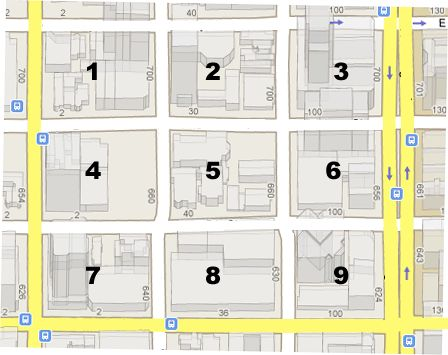
\includegraphics[width=3.0in]{blocks.jpg}
    \caption{Blocks in a city; a block has more faces for each street; a street block is the spacial unit for the SFpark data; image source\cite{blocks_source}}
    \label{fig:blocks}
\end{figure}

Time-wise the data is structured per full hour, i.e. as integers from 0 to 23. For this experiment only a fraction of the whole available data is used, more precisely only the \textbf{blocks}, \textbf{times of measurement} and \textbf{occupancy rates}. This however is enough in order to detect patterns of occupancy-time correlations, e.g. blocks that have a peak in the morning and evening, blocks that are peaking only in the evening and weekends, etc.
\vspace{2mm}

The platform on which the experiment was run is the Machine Learning service \url{http://bigml.com}. The site initially allows processing datasets of up to 16MB for free, by running up to 2 parallel tasks in the cloud. Soon after starting to use it, I received a free update for crunching 1GB datasets for 1 month. The ML methods available are Classification, Regression, Cluster Analysis, Anomaly Detection and Associative Discovery.
\vspace{2mm}

Uploading data sources can be done through the service itself or from another cloud storing service, in case of larger files. I made an Amazon S3 account and loaded my data sources there first. Then I provided the URL to the source to load it in BigML (see figure~\ref{fig:amazon_s3}).

\begin{figure}[!ht]
    \centering
    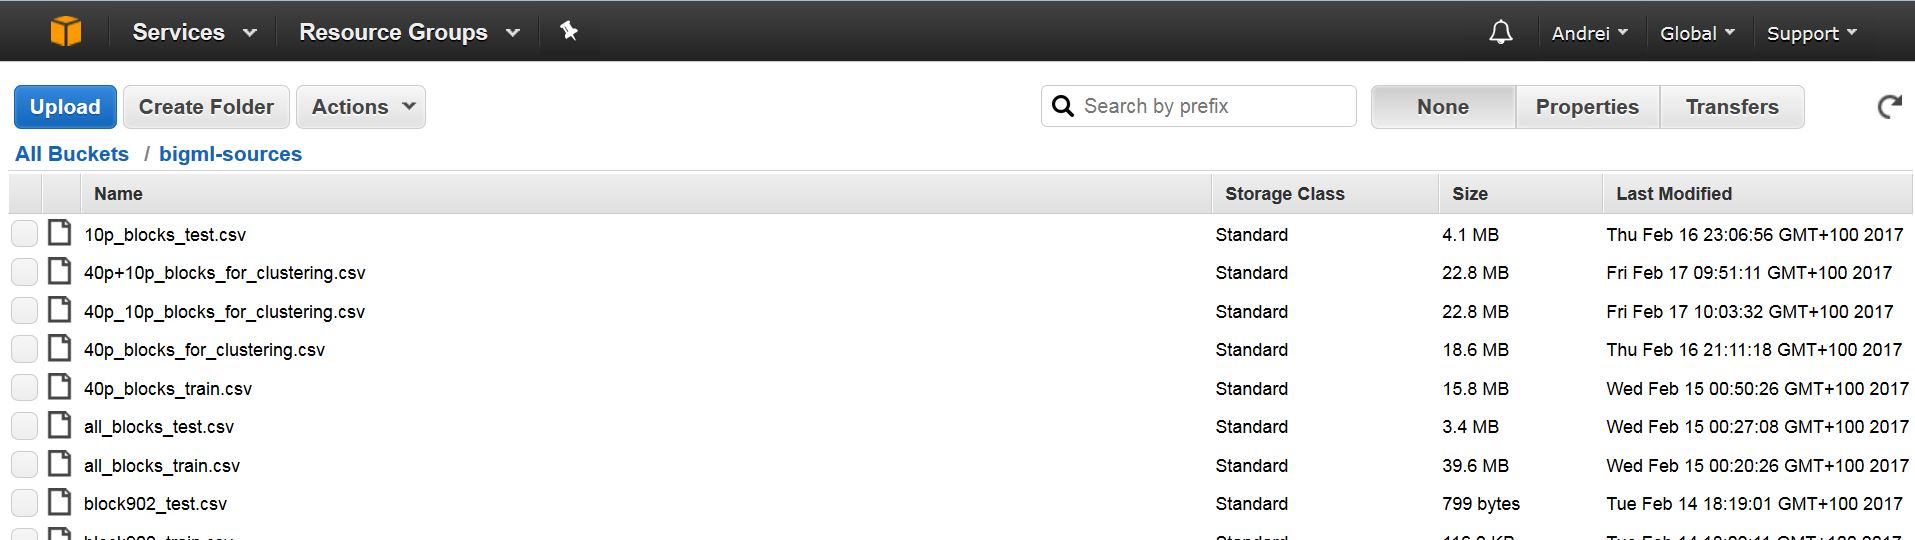
\includegraphics[width=4.0in]{amazon_s3.jpg}
    \caption{My Amazon S3 account with directory and file layout}
    \label{fig:amazon_s3}
\end{figure}

\section{Data Preprocessing}
\label{sec:Data_Preprocessing}
The dataset to be loaded on the BigML platform will contain blocks, times and occupancy rates. Since we are developing a prediction, for simplicity select prediction in 1 hour. Hence, the following pieces of information need to be extracted from SFpark data:
\begin{itemize}
\item block id
\item date and time 
\item occupancy (current)
\item occupancy in 1 hour 
\end{itemize}
\vspace{2mm}

It turns out that the first two points are readily available in the SFpark parking occupancy dataset. The occupancy values are, however, indirectly represented by \textbf{Total occupied seconds}, \textbf{Total vacant seconds} and \textbf{Total unknown seconds} (see figure~\ref{fig:sfpark_occupancy_screenshot}). 
\vspace{2mm}

\begin{figure}[!ht]
    \centering
    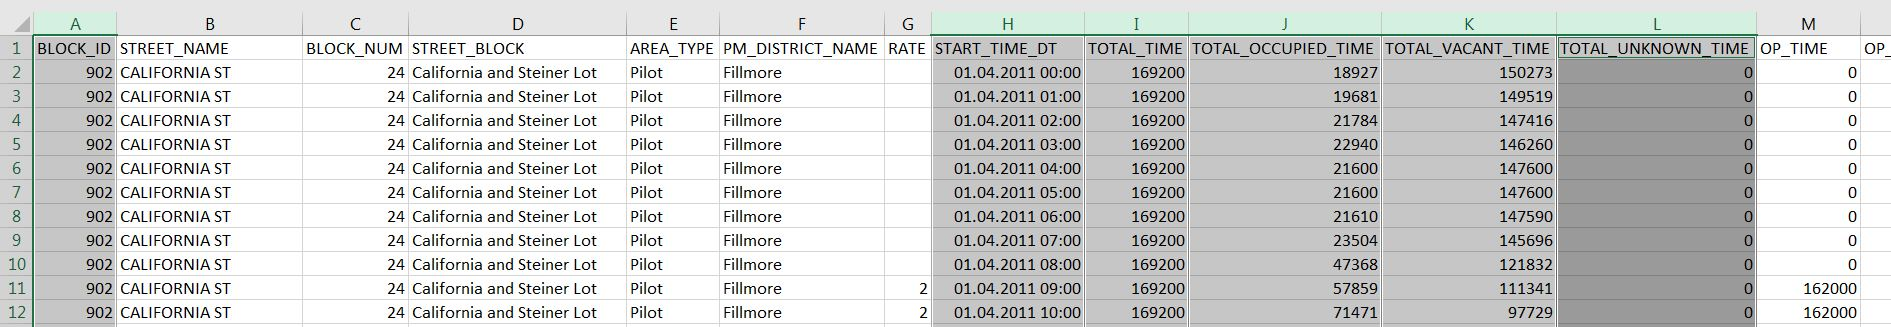
\includegraphics[width=5.0in]{sfpark_occupancy_screenshot.jpg}
    \caption{Extract of the SFpark occupancy spreadsheet; selected colums are interesting here}
    \label{fig:sfpark_occupancy_screenshot}
\end{figure}

Each of these values is the sum in seconds of all the sensors on the respective block that reported car occupation, vacancy or unknown status. The latter basically means that the respective sensor was out of order at that time. Following the SFpark evaluation guide, to calculate the occupancy rate, the unknown time will not be included in the total time at the denominator:
\vspace{2mm}

$$
\text{Occupancy Rate} = \frac{\text{Total occupied}}{\text{Total occupied} + \text{Total vacant}}
$$

As far as time is concerned, we want to detect patterns with regard to time of day, day of week and perhaps even calendar week. Therefore these values are extracted from the provided date+time stamp. A snapshot of the final dataset to be uploaded in BigML looks as follows. It contains about 1,048k lines and is 51MB large (see figure~\ref{fig:dataset_screenshot}).
\vspace{2mm}

\begin{figure}[!ht]
    \centering
    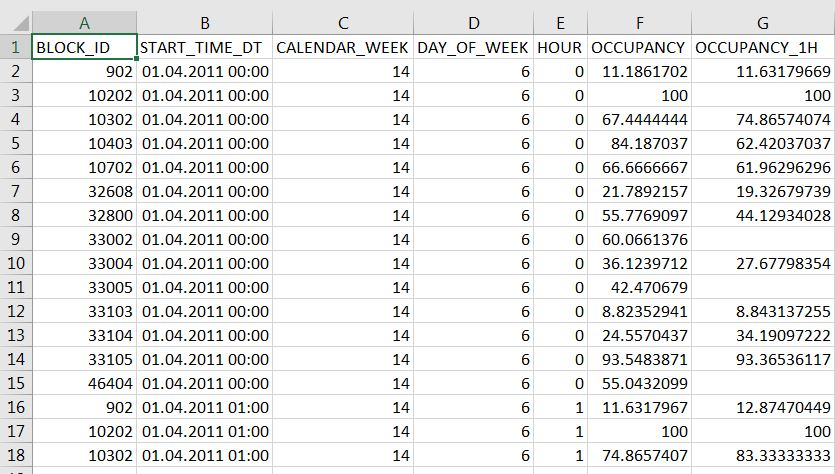
\includegraphics[width=4.0in]{dataset_screenshot.jpg}
    \caption{Extract of the CSV file that is ready for processing; notice that some occupancy in 1h values are not available due to temporary not functioning sensors}
    \label{fig:dataset_screenshot}
\end{figure}

\section{Building the models}
\label{sec:Building_the_models}
In the first step, a CSV file is loaded (possibly via Amazon S3) in BigML under \textbf{Sources}. At this point, one can configure the datatypes of the fields. Blocks is Categorial, Date+Time stamp is Datetime, while all the others are numerical (see figure~\ref{fig:bigml_source_field_datatypes}). 
\vspace{2mm}

\begin{figure}[!ht]
    \centering
    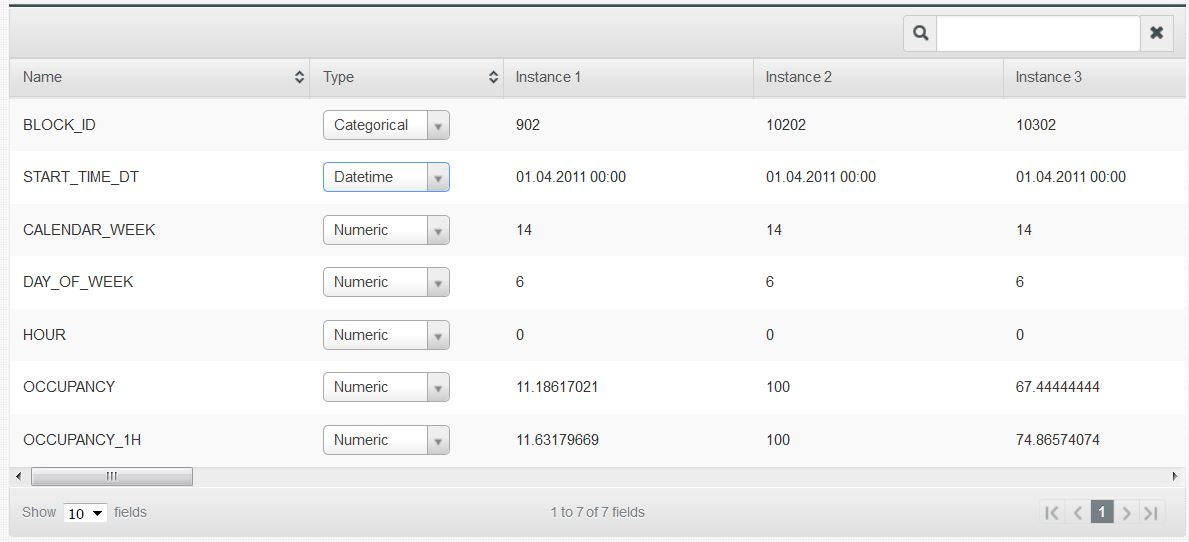
\includegraphics[width=4.0in]{bigml_source_field_datatypes.jpg}
    \caption{Setting datatypes for the fields in the Sources area in BigML}
    \label{fig:bigml_source_field_datatypes}
\end{figure}

Next step is the creation of a proper dataset, that BigML internally uses for further operations. In our case it is identical to the source (see figure~\ref{fig:bigml_dataset}).
\vspace{2mm}

\begin{figure}[!ht]
    \centering
    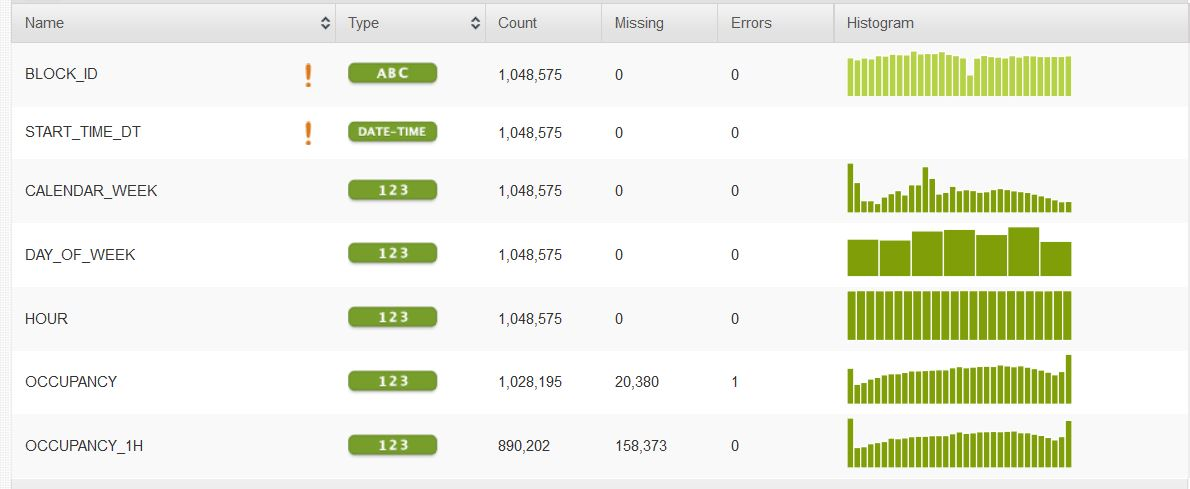
\includegraphics[width=4.0in]{bigml_dataset.jpg}
    \caption{The view on the dataset in BigML}
    \label{fig:bigml_dataset}
\end{figure}

From the dataset one can start a K-means clustering with 8 clusters. The fields to be taken in account for clustering are \textbf{calendar week}, \textbf{day of week}, \textbf{hour} and \textbf{occupancy}. Missing values will be filled with a default value. The result is displayed as follows (see figure~\ref{fig:bigml_clusters}).
\vspace{2mm}

\begin{figure}[!ht]
    \centering
    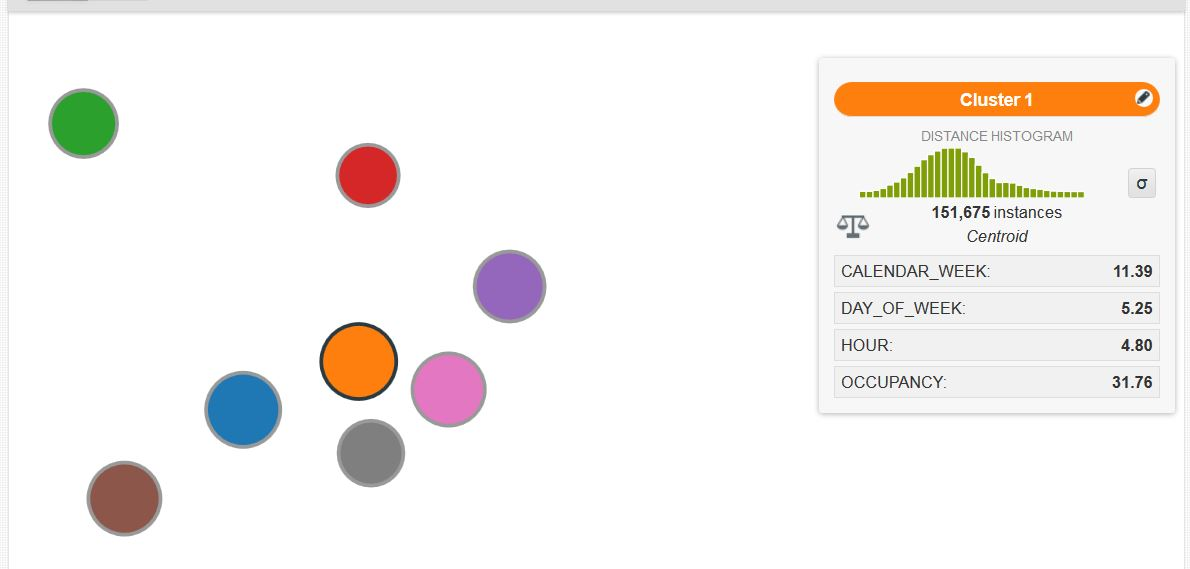
\includegraphics[width=4.0in]{bigml_clusters.jpg}
    \caption{Clusters visualisation in BigML}
    \label{fig:bigml_clusters}
\end{figure}

The assumption here is that nearby clusters have a similar time-occupancy pattern. The following steps will build upon this assumption. In case the assumption is false, the results should reveal this fact.
\vspace{2mm}

A prediction model is built for the center cluster (in the figure above, Cluster 1). The target variable is \textbf{Occupancy 1H}. BigML uses decision trees for this operation (see figure~\ref{fig:bigml_decisiontree}).
\vspace{2mm}

\begin{figure}[!ht]
    \centering
    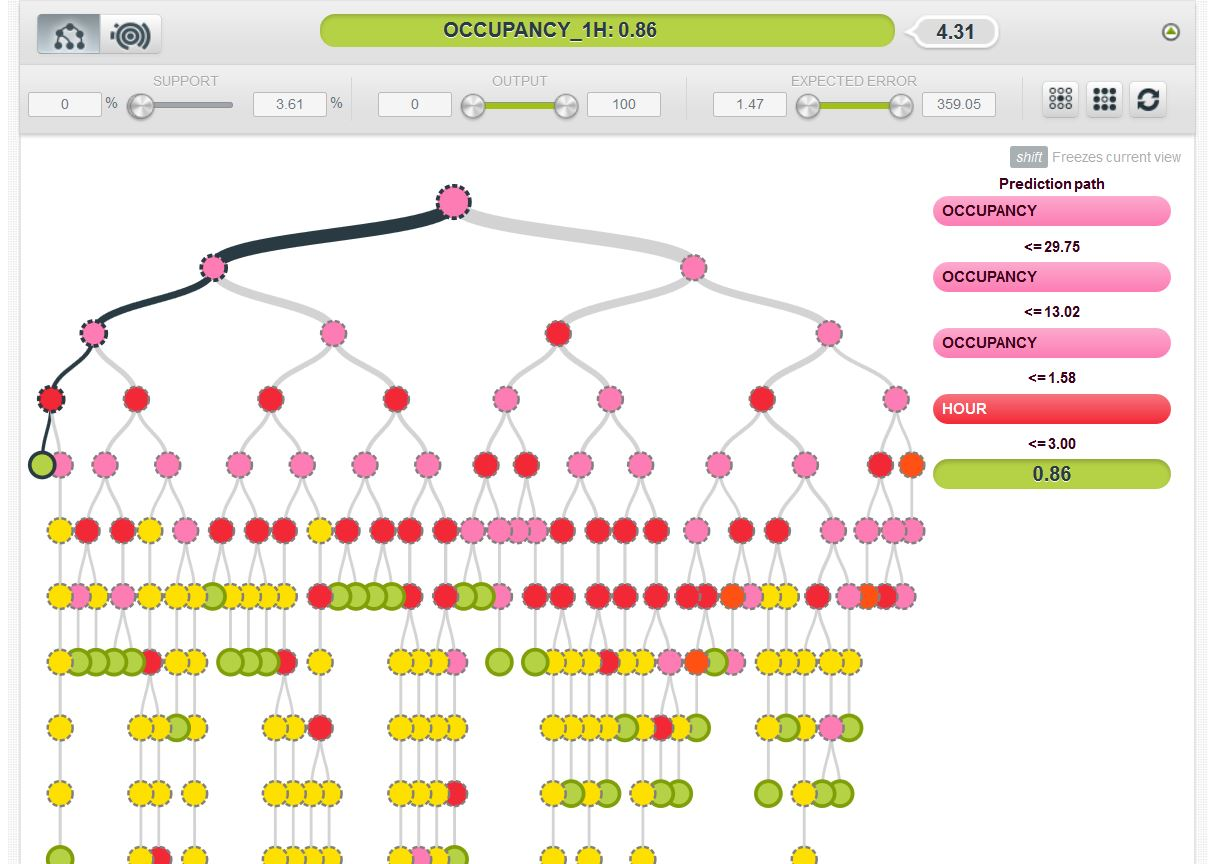
\includegraphics[width=3.0in]{bigml_decisiontree.jpg}
    \caption{Visualisation of a prediciton model as a decision tree in BigML}
    \label{fig:bigml_decisiontree}
\end{figure}

This model is used for prediction on the other datasets represented by the surrounding clusters. Their \textbf{occupancy in 1h} values are ignored during the process and will be used afterwards to calculate the prediction accuracy. 
\vspace{2mm}

\section{Evaluation}
\label{sec:Evaluation}
The accuracy is calculated as the average absolute difference between the measured \textbf{occupancy in 1h} and the predicted one:
\vspace{2mm}

$$
\text{Model Prediction Error} = \frac{\sum_{\text{record}}|\text{Ocuppancy1h}_\text{real} - \text{Occupancy1h}_\text{predicted}|}{\text{number of records}}
$$

Here is the error calculated for each cluster, as described above:
\vspace{2mm}

\begin{figure}[!ht]
    \centering
    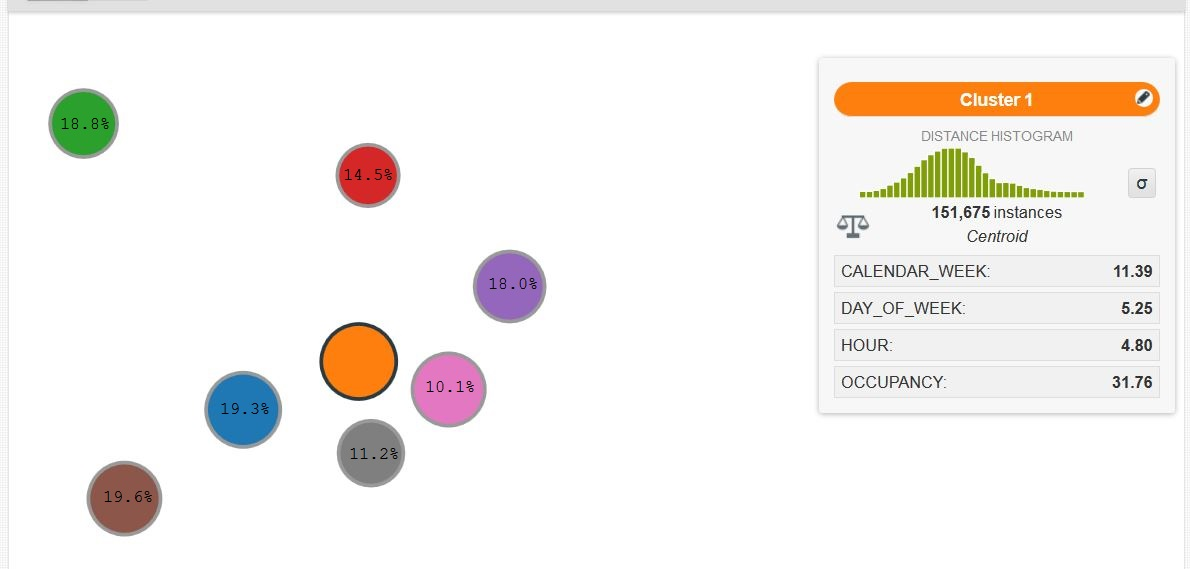
\includegraphics[width=5.0in]{cluster_errors.jpg}
    \caption{Annotated cluster image with the aveage absolute error for each cluster dataset apart from the center cluster}
    \label{fig:cluster_errors}
\end{figure}

In looking at this result, there is a slight tendency to be seen: the further away a cluster is from the center cluster, the larger the error when applying the model of its central cluster on its dataset. I would have wished that this tendency is clearer, however, by adding other attributes to the datasets, e.g. parking price, traffic, weather and, of course, GIS metadata, such a tendency may become clearer.
\vspace{2mm}

I also run another comparison. I created a dataset with 90\% of the data, created a prediction model using the same Decision Tree method and having \textbf{occupancy in 1h} as target variable. I then applied it to the rest 10\% of the data. The prediction error in this case was 9.3\%. Note that the data is split time-wise, so that blocks will be present in both training and test datasets. 
\vspace{2mm}

Despite the general model delivering a better result, I believe that by enriching the datasets with other attributes, the smaller clusters will build more fitted models that will improve on the error of the whole model.

\section{Conclusion}
\label{sec:Conclusion}

By using clustering as a pre-processing step, a similarity function is internally computed between the future prediction models. This is equivalent to the similarity measure described in the thesis idea from a previous document.

This experiment has shown that such an approach delivers decent results when the models contain just basic attributes. By adding more attributes, the clustered models will be more accurate and I believe that their preciseness will surpass the one of a general prediction model.

\nocite{*}

\printbibliography

\end{document}